\documentclass{ieicej}
%\documentclass[invited]{ieicej} % 招待論文
%\documentclass[comment]{ieicej} % 解説論文
\usepackage{graphicx}
%\usepackage{latexsym}
%\usepackage[fleqn]{amsmath}
%\usepackage[psamsfonts]{amssymb}

\input comment.sty


\setcounter{page}{1}

\field{B}
\jtitle{分散OS開発学習キット LP49}
\etitle{An open source kit for developing and studying a distributed OS ``LP49''}
\authorlist{%
 \authorentry{丸山 勝巳}{Katsumi MARUYAMA}{NII}
 \authorentry{佐藤 好秀}{Yoshihide SATO}{NII}[Hitachi]
 %\authorentry[メールアドレス]{和文著者名}{英文著者名}{所属ラベル}
 %\authorentry{和文著者名}{英文著者名}{所属ラベル}[現在の所属ラベル]
}
\affiliate[NII]{国立情報学研究所}{National Institute of Informatics}
%\affiliate[Hitachi]{日立製作所}{Hitchi Co. Ltd.}
%\paffiliate[]{}
\paffiliate[Hitachi]{日立製作所}

\begin{document}
\begin{abstract}
OSはシステムの性能(機能・効率・信頼性)のみならず
プログラム開発コスト(開発しやすさ,開発期間・拡張性など)を大きく左右する.
信頼性向上の鍵はシンプル化であり,
目的に最適なシンプルな分散OSの開発・学習キットは意義がある.
%
開発・学習用OSは,重要機能を全て含み,構成が簡明で,容易に機能追加でき,
プログラム規模も小さいことが望まれる.
本報告では,マイクロカーネルとマルチサーバを基本とした
分散OS学習・開発キットについて紹介する.

\end{abstract}

\begin{keyword}
分散OS, L4, Plan9, マイクロカーネル,マルチサーバ,コンポーネント 
\end{keyword}
\begin{eabstract}
  Control systems (e.g. embedded systems, home servers) are becoming more and more sophisticated, 
  networked and complex. 
  Software dependability and productivity are the first concern of their design,  
  and Operating Systems play very important roles.
  It will be nice to have a distributed OS kit for studying and developing.
  LP49 is a component-oriented OS with micro-kernel and multi-server architecture,
  and suitable for this purpose. 
\end{eabstract}
\begin{ekeyword}
Distributed OS, L4, Plan9, Micro-kernel, Multi-server, Component 
\end{ekeyword}

% 表題などの出力
\maketitle

%}{

% 本文はここから始まる
\section{はじめに}

  今や組み込みシステムやホームサーバには,NW接続された多様な機器を連携動作させる
分散処理機能が必須である.
OSはシステムの性能(機能・効率・信頼性)のみならず
プログラム開発コスト(開発しやすさ,開発期間・拡張性など)を大きく左右する.
信頼性向上の鍵はシンプル化であり,
目的に最適な分散OSを作りたい人にはシンプルな分散OS開発キットは意義がある.
%
  また,OSはソフトウェア技術の集大成であり,最高のソフトウェア教材である.
学習用分散OSは,重要機能を含み,構成が簡明で,容易に機能追加でき,
プログラム規模も小さいことが望まれる.
学習用OSとしては,Minix が大変すぐれているが,
残念ながら分散処理機能は目的としていない.

このように,分散OSの適切な開発・学習キットは大変意義が高い.
本報告は,以上の観点から分散OS開発・学習キットLP49について紹介する.

%}{

\section{本OS開発学習キットの意図}\label{sec:Enum}\label{sec:item}

シンプルな分散OS開発学習キットに向けて以下を目指している.

%\begin{itemize}

%\item 
{\bf 制御システム(組込みシステム) やサーバに適したシンプルなOS:} 
      制御用,サーバ用に必要な機能をもったコンパクトな分散OS.
    
%\item 
{\bf マイクロカーネル+マルチサーバ構成による障害に対する頑強性の強化:} 
    モノリシックOSでは部分障害 (例えばドライバのバグ) でもシステムクラッシュを導きがちである.
    障害が生じても波及範囲を閉じ込めて部分再開を可能とするためには,
%    以下の内容の
    マイクロカーネル+マルチサーバ構成の OSが有利である.
%    (a) マイクロカーネル以外は,全てユーザモード(プロセッサの非特権命令)で実行させる.
%    (b) 名前空間管理,ファイルサービスなどのいわゆるOSサービスは,
%        個別のユーザモードプロセスとして実現し,個別再開を可能とする.
%    (c) デバイスドライバ (OSクラッシュの原因の7割はドライバと言われる)も,
%        ユーザモードで動作させる.
    
%\item 
{\bf 拡張性の強化:} 
    機能追加はユーザモードプロセスの追加などにて容易に行えるようにする.

%\item  
{\bf システム連携の機能:} 
   最近の組込みシステムには,
   分散リソースの体系的な管理と制御,
   ノード間での名前空間の可視化,
   環境変数を含む動作環境の連携など
   従来の分散OSを越えた機能が要求される.

    また,分散処理のプロトコルは提供できる機能と性能を決定するが,
  独自プロトコルは普及させることは難しい.
  Plan9\cite{plan9}の{\bf 9Pプロトコル}は,
  {\tt attach(), walk(), open(), create(), 
  read(), write(), clunk(), remove(), stat()}
  等のメッセージからなり,
  低レベル制御も可能で融通性が高いので,これを採用した.


%\item 
{\bf プログラム開発の容易化:} 
   モノリシックOSは,カーネル(特権)モードで動いている.
   カーネルモードプログラムは,開発に高いスキルが必要でデバッグが大変難しい.
   その上,小さなバグでもシステム全体がクラッシュしかねない.
   本OSでは,マイクロカーネル以外は全てユーザモードプログラムとし,
   ほとんどのサービスはユーザモードプロセスの追加で実現でき,
   デバイスドライバもユーザモード化した.
   これにより,プログラム開発が容易化・効率化される.

%\item 
{\bf L4\cite{L4}とPlan9\cite{plan9}のソースコード活用:}   
    OS全体をスクラッチから作るには,膨大な工数を要する.
    Karlsruhe大学の L4 マイクロカーネルは, 
    簡潔で優れたスレッド・メッセージ性能を持っている.
    また,Bell研で開発された Plan9 は,融通性の高い分散処理を実現している.
    かつ両者ともオープンソースであるので,ソースコードを活用して
    工数削減をはかった.
    
%\item 
{\bf 使い慣れたプログラム開発環境:} 
      OS を学習したり自前のOSを開発したい人に手頃なソースコードを提供するとともに, 
  使い慣れたGNU環境でプログラム開発からテスト走行までできるようにした.

%\end{itemize}    

%}{

\section{プログラム構成}

      LP49 は,図 \ref{fig:LP49general} に示すように以下の階層からできている.

\begin{figure*}[tb]
  \begin{center}
   %\epsfxsize=340pt
   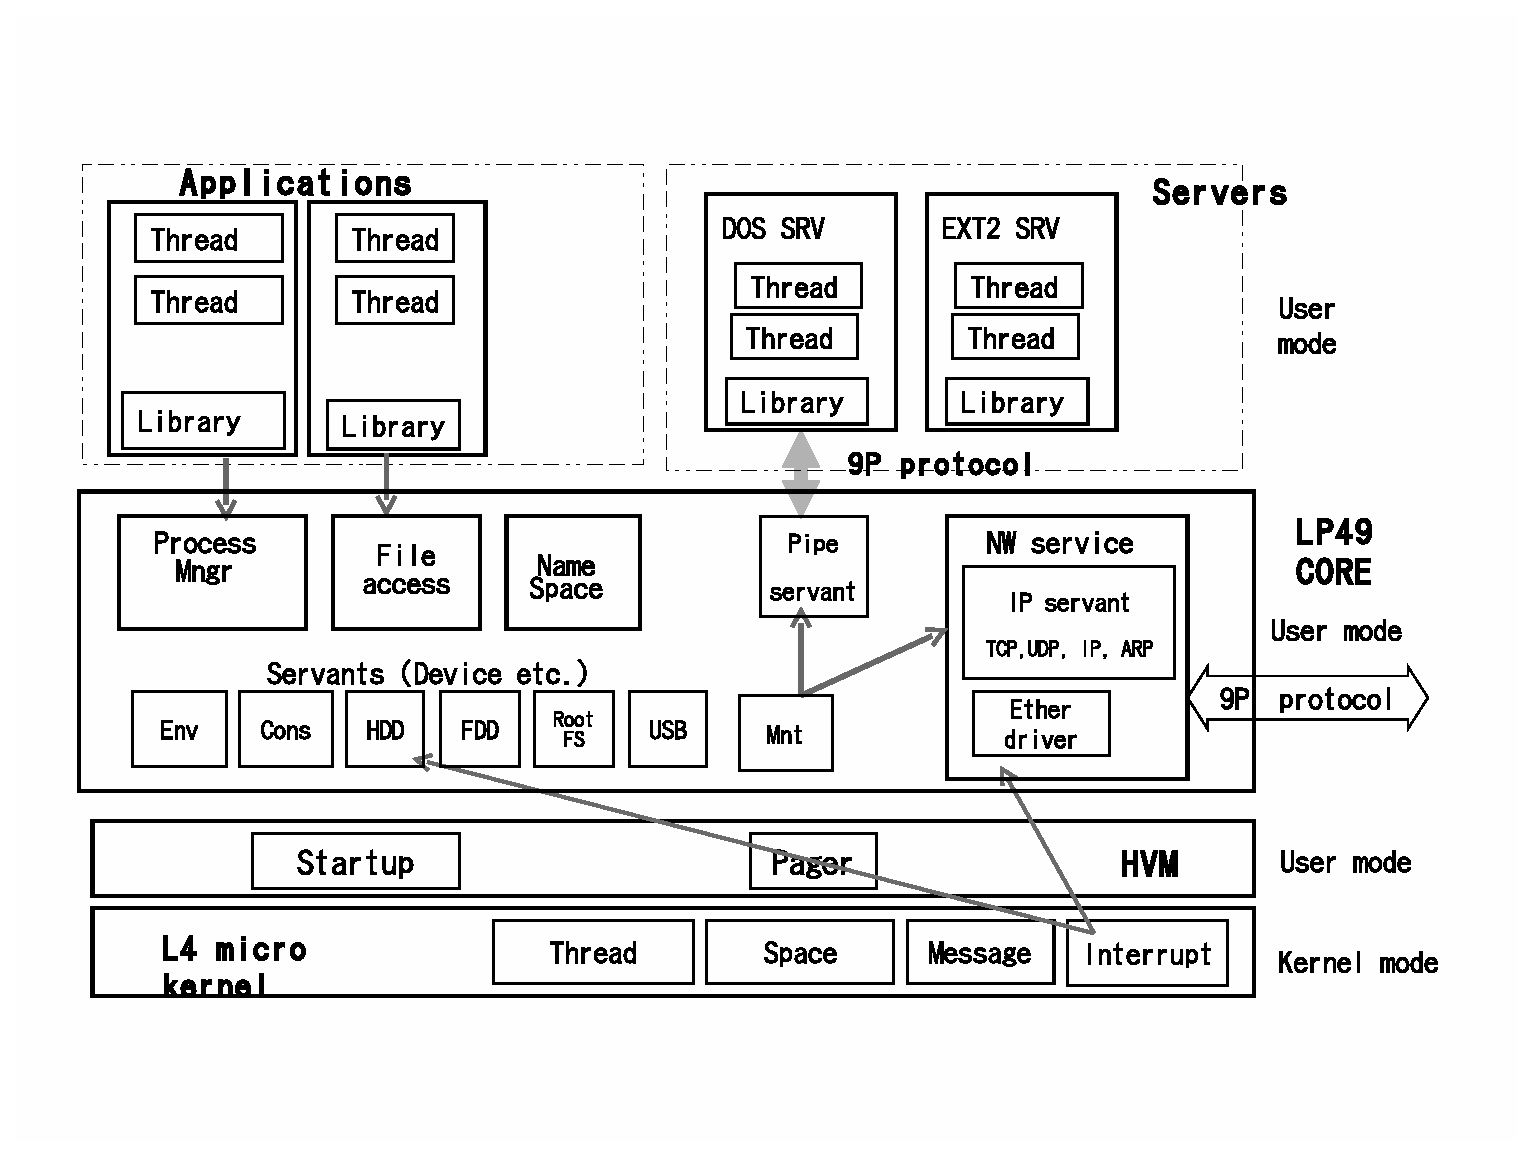
\includegraphics[width=130mm]{../fig/LP49general.eps}
    \caption{LP49全体構成}
    \label{fig:LP49general}
    \ecaption{LP49 structure}
  \end{center}
\end{figure*}


%\begin{itemize}
%\item 
{\bf マイクロカーネル階層  (カーネルモード): }
     L4 マイクロカーネルそのものであり,唯一カーネルモードで動作している.
     マルチスレッド,タスク(=プロセス)論理空間,スレッド間通信,ページマップの
     機能を提供している.
    
%\item 
{\bf HVM 階層 (ユーザモードプロセス): }
     ユーザモードで走るL4プロセスである.
     LP49 の立ち上げ,スレッド制御と論理空間制御,
    並びにページフォールトの対処を行うスレッド ({\tt Pager}) を持っている.
%
    L4マイクロカーネルは,スレッドの実行中にpage faultが生じると,
    本{\bf Pager}スレッド にpagefaultメッセージを送る.
   {\tt Pager} は pagefault メッセージを受信すると,
   適切な実ページを決定し L4の page map機能を使って割り当てる.
   なお,応用プログラムは, page faultの処理をHVMの{\tt Pager}に行わせても良いし,
   自分独自のPagerを記述することも可能で,
   ページキャッシュ,トランザクションメモリなど
   融通性の高いメモリ管理も実装できる.
%
    HVMという名前は,将来 Hypervisor Monitor 階層として Virtual Machine に発展させることを
    意図したが,現時点ではその機能は持っていない.

    
%\item 
{\bf Core階層  (ユーザモードプロセス): }
     APLプロセスからシステムコール (実際にはメッセージ) を受けて,
    必要ならばサーバプロセスに仕事を依頼して,
    要求された処理を行う.
   つまり,プロセスのシステムコールに対してはサーバ,
   サーバプロセスに対してはクライアントとして機能する.
%   
    プログラムは,ユーザモードつまり非特権モードで走るので,安全性が高い.
    デバイスドライバもここに含まれる.

    
%\item 
{\bf サーバ階層 (ユーザモードプロセス): }
     OSサービスを行うファイルサーバー類も普通の応用プログラムも,
     同等のユーザモードプロセスである.
    ファイルサーバは,後述の様に 9P プロトコルを話せる点がちがうだけである. 
%\end{itemize}

%%%
\section{サービスと抽象ファイル}

\subsection{サービス提供:サーバとサーバント}

  OSが提供するサービスには,
  Dosファイルサービス,Ext2ファイルサービスといった高位サービスと,
  ハードウェア駆動,モジュール間通信,NW接続,サーバ登録簿といった低位サービス
  とがある.

  前者は,個々に独立性が高く,規模も大きくなりがちなので,
  サービス毎にユーザモードプロセスとして実現した.これを{\bf サーバ}と呼ぶ.
  サーバはメッセージインタフェースなので,ローカルでもリモートでも同等に使える.
  ユーザモードプロセスなので,プログラム開発の容易化のみならず,
  障害時もそのサーバだけを停止・再開することで耐障害性も強化される.

  後者は共通機能的で,より実行速度が重視されるので,
  独立したプロセスとはせず LP49core内のモジュールとして実装することとした.
  このモジュールを{\bf サーバント}と呼んでいる.
  サーバントは,統一インタフェースを持つコンポーネントである.
  機能的には,同一サービスをサーバとして実装することも
  サーバントとして実装することも可能である.

   サーバもサーバントも,
   内部リソースを登録する名前空間 (directry tree)を持っており,
   プロセスはそれを自分の名前空間にマウントすることにより,
   普通のファイルインタフェースで目的リソースにアクセスして,
   内容の読み書き・制御を行える.
   プログラム構造的にも優れたコンポーネントと言える.

{\bf\flushleft (1) サーバント}

    サーバントはハードウェアデバイス, サーバ登録簿,環境変数記憶,
  pipe, プロトコルスタックなど低位サービスを提供する.
  サーバントはLP49coreプロセス内のモジュールであり,
  attach(), init(), open(), read(), write(),,, といったプロシージャインタフェース
  で呼ばれる.
%
  各要素はサーバントの名前空間に登録されており,
  ファイルインタフェースで操作できる.
  サーバントは \verb|#+<英字>| の形式のサーバント識別子をもつ.
  代表的サーバントを以下に示す.括弧内は サーバント識別子である: 
%
{\small
% \begin{quote}
     コンソール(\verb|#c|), ハードディスク(\verb|#S|), フロッピーデバイス(\verb|#f|), 
     環境変数 (\verb|#e|), サーバ登録簿(\verb|#s|), サーバマウント(\verb|#M|), 
     Etherドライバ(\verb|#l|), 
     プロトコルスタック(\verb|#I|), Pipe(\verb$#|$), ルートファイルシステム(\verb|#R|), 
     USBホストコントローラ(\verb|#U|), VGAコントローラ(\verb|#v|),,,
% \end{quote}
}

``{\tt bind}''コマンドにより,サーバントをプロセスの名前空間に結合することにより,
プロセスからサーバントにアクセスできるようになる.

%  \verb|bind  サーバント識別子 マウントポイント|  
  {\tt bind}  {\em\small サーバント識別子}  {\em\small マウントポイント}  

{\bf\flushleft (2) サーバ}

  サーバはサービスごとに独立したユーザモードのプロセスであり,
  9Pメッセージ (9Pプロトコル)を受信してサービスを実行する.
  LP49coreとサーバの間で9Pメッセージを運ぶ接続を{\bf サーバリンク}と呼んでいる.
  サーバリンクは,
  ローカルサーバの場合は pipe (LP49の pipe は 双方向である),
  リモートサーバの場合は TCP/IP 接続を用いる.
%
  各サーバのサーバリンクを登録しておくデータベースが {\bf サーバ登録簿}である.
  サーバ登録簿はサーバントの一つ(\verb|#s|)で, 
  立ち上げ時に ``{\tt /srv}``として接続されている.
  クライアントは,サーバ登録簿から目的のサーバを見つけて,
  サーバリンク名(ex. {\tt /srv/dos}) を自分の名前空間にマウントする.
  これにより,サーバの名前空間がクライアントの名前空間に接続され,
  普通のファイルインタフェースでアクセスできるようになる.

%  \verb|mount サーバリンク マウント位置 付加指定| 
  {\tt mount}  {\em\small サーバリンク}  {\em\small マウント位置}  {\em\small 付加指定} 


%%%
\subsection{抽象ファイルオブジェクト}\label{sec:VF}

Plan9と同様,LP49 では殆どのリソースを``ファイル''として抽象化している.
個々の``抽象ファイル''は,サーバント内あるいはサーバ内に存在し,
名前空間(directory tree)に登録されている.

オブジェクト指向の観点からは,図 \ref{fig:VirtualFileObject}に示すように
``抽象ファイル''はインスタンスオブジェクト,
``サーバント定義''はクラス定義に相当する.
各サーバントは同一のインタフェースを有する.

\begin{figure}[tb]
  \begin{center}
   %\epsfxsize=340pt
   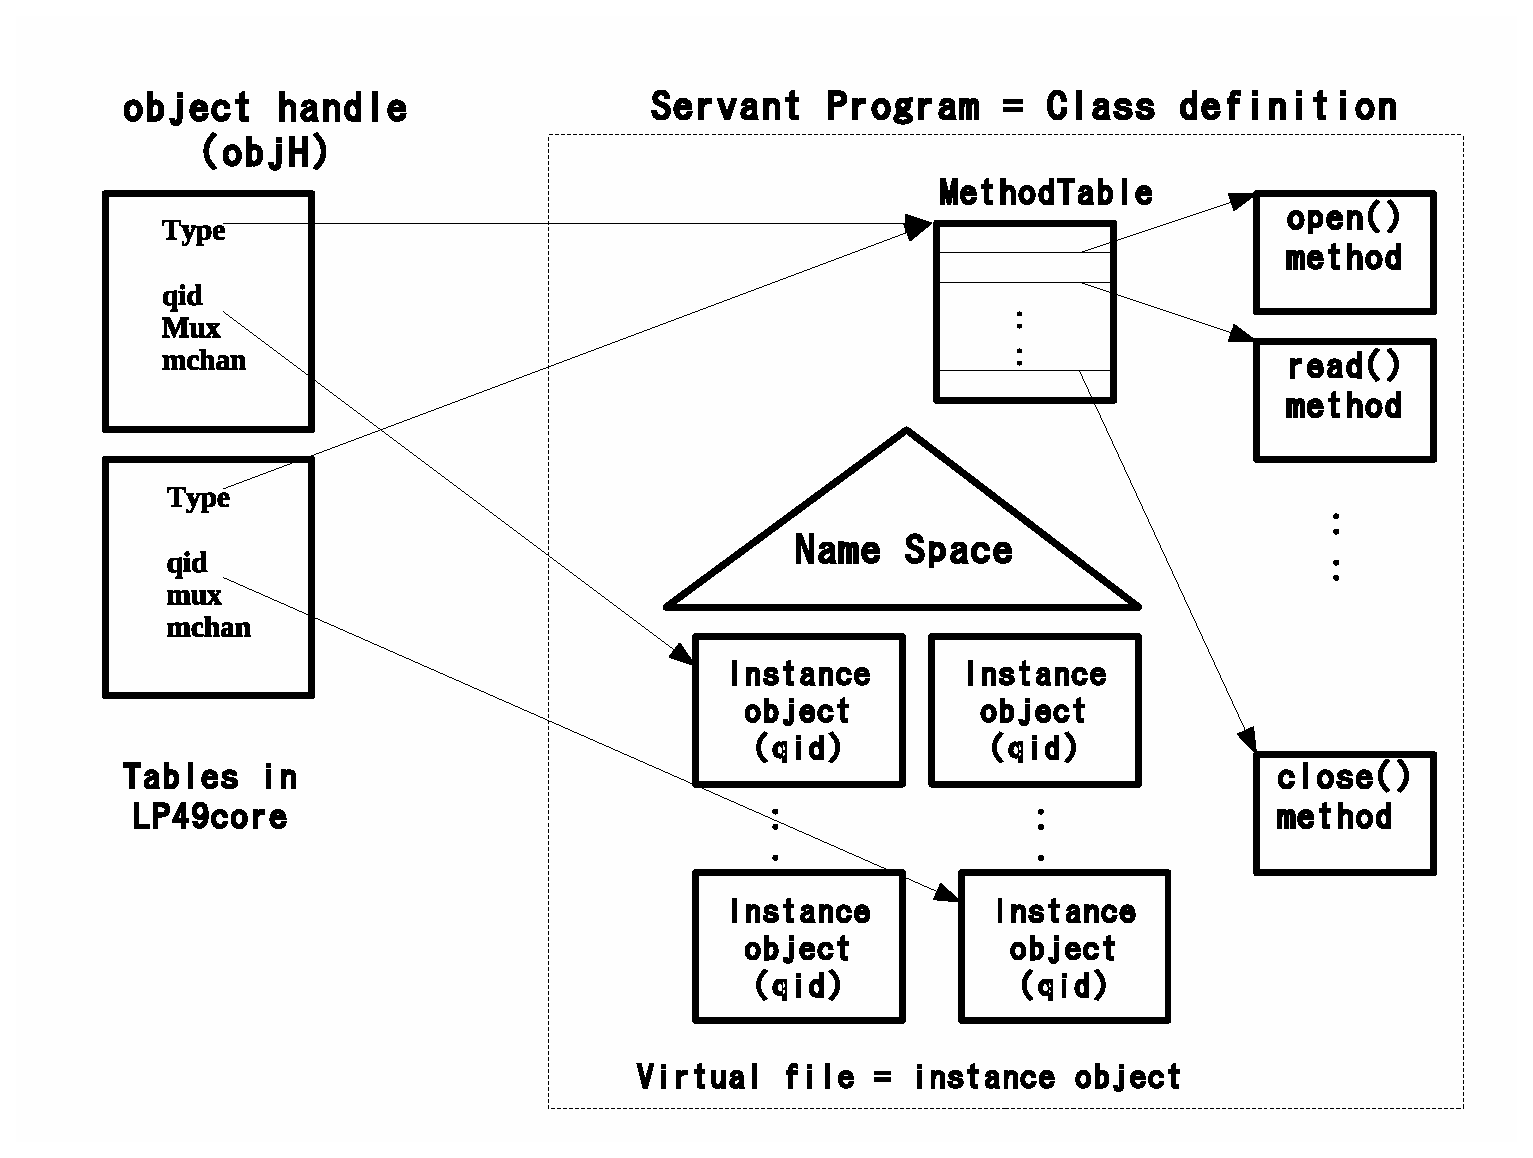
\includegraphics[width=75mm]{../fig/VirtualFileObject.eps}
    \caption{仮想ファイルのオブジェクトモデル}
    \label{fig:VirtualFileObject}
    \ecaption{Virtual file object model}
  \end{center}
\end{figure}


\begin{itemize}
\item  各サーバントプログラムはクラス定義に相当し,
  attach(), init(), open(), read(), write(),,, 等のメソッドコードを持ち,
  メソッドテーブルを介して呼ばれる.
\item  ``抽象ファイル''は,インスタンスオブジェクトであり,
   サーバントの名前空間に登録されている.
   以下では {\bf VF(抽象ファイル)オブジェクト}と呼ぶ.

\item  VFオブジェクトは,qidという値によりサーバント内でユニークに識別される.
       qid は Unix の inode番号に相当する.

\item  一般のオブジェクト指向言語と違って,同一クラス(サーバント)内でも
       各VFオブジェクトのデータ構成は同一とは限らない.
       各メソッドはVFオブジェクトのqidから,そのデータ構成を判定し,
       対応した処理を行う.

\end{itemize}


  LP49core内では,VFオブジェクトは{\bf オブジェクトハンドル}({\tt objH})
を介してアクセスされる.
オブジェクトハンドルは,サーバント識別情報({\tt typeフィールド}), 
VFオブジェクトのqid ({\tt qidフィールド}), 
その他の管理情報が載ったテーブルである
\footnote{ Plan9 ソースコードを元に修正したので,
プログラム上ではこのテーブルのタイプ名はChan(nel)となっている}.
LP49coreは,
オブジェクトハンドルの{\tt typeフィールド}からサーバントの各メソッドをアクセスし,
{\tt qidフィールド}からインスタンスを決定する.
%
ここではVFオブジェクト $\alpha$ を指すオブジェクトハンドルを
``{\tt objH\{$\alpha$\}}''と表記する.

オブジェクトハンドルは,対象を{\tt open(), create()}した時や,
change directory した時に割り当てられ,
参照カウンタが 0 になったときに消去される.



%%%%
\section{システムコールの仕組み}

\subsection{サーバントによる処理}

  システムコールは,モノリシックOSでは一般にトラップを用いるが,
マイクロカーネルOSではメッセージ通信を用いる.
システムコールの仕組みを図 \ref{fig:LP49syscall}に示す.

\begin{figure}[tb]
  \begin{center}
   %\epsfxsize=340pt
   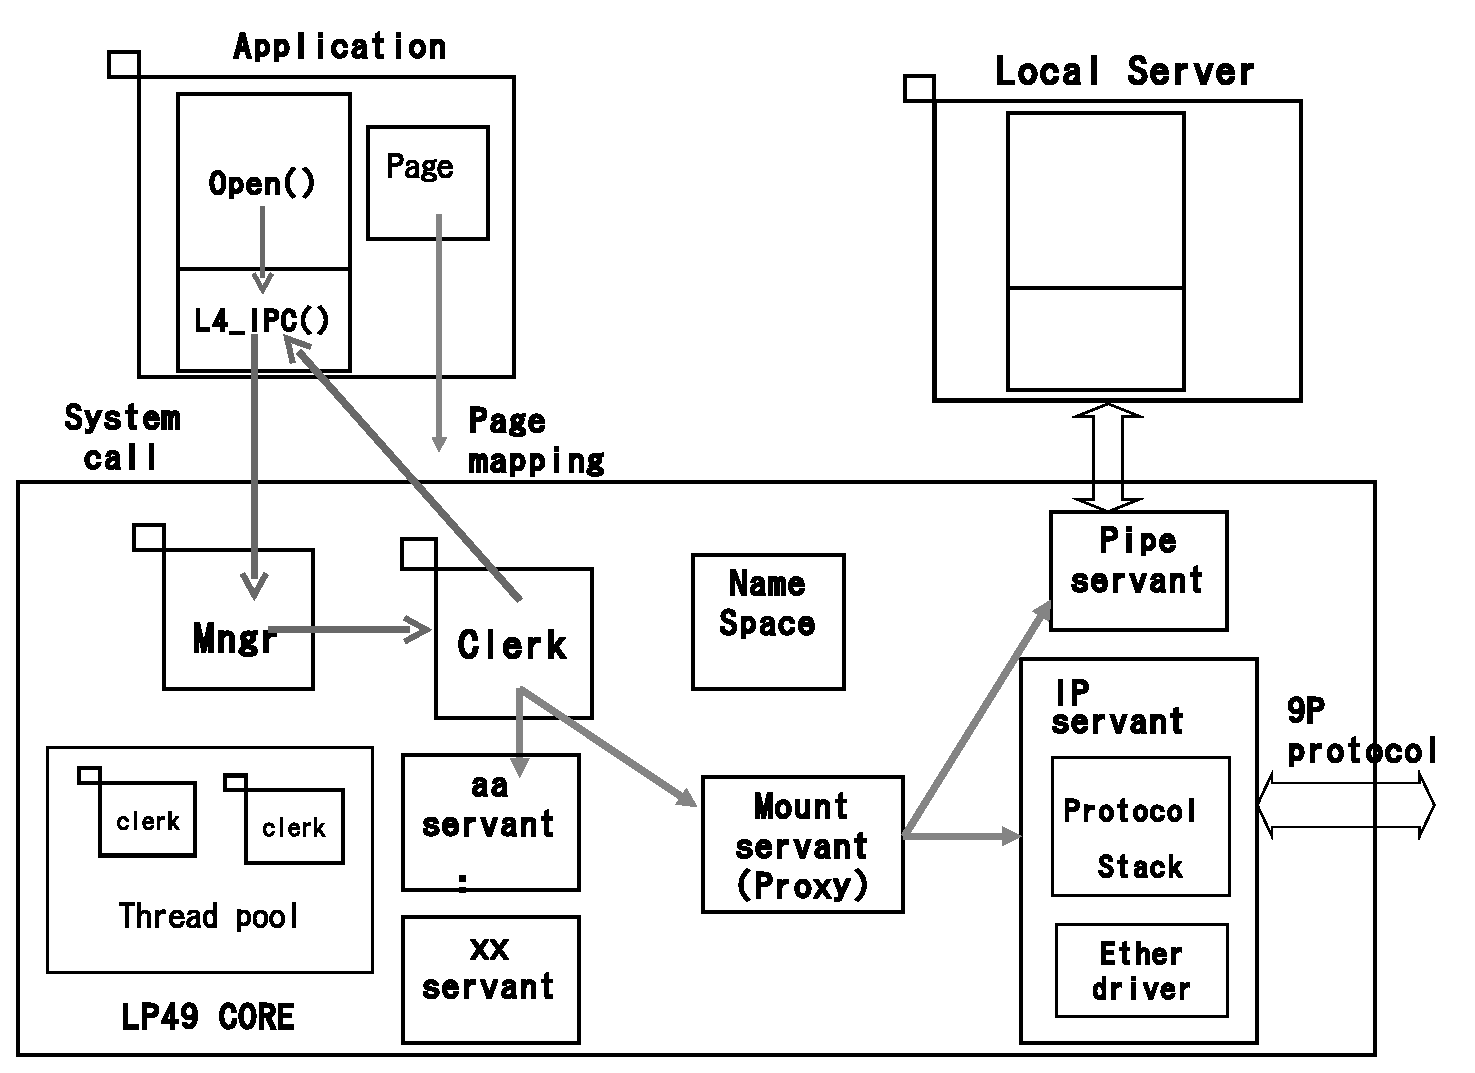
\includegraphics[width=70mm]{../fig/LP49syscall.eps}
    \caption{システムコール}
    \label{fig:LP49syscall}
    \ecaption{System call}
  \end{center}
\end{figure}

{\bf (1) ライブラリによるL4メッセージ化}

  APLのシステムコールは, 使い慣れた関数呼び出し ({\tt open(...), read(...), write(...)} 等) 
  である.
  ライブラリは,これを L4 メッセージに変換して LP49core に送り,返答メッセージを待つ.
  APLとLP49coreは別論理空間なので,アドレス引き継ぎは使えない.
  システムコールの引数引き継ぎには,小サイズのデータはL4メッセージの値コピー,
  バッファー域はL4メッセージのページマップ機能を利用した.


{\bf (2) LP49core マルチスレッドサーバ}

    LP49coreは,APLのシステムコール処理に対してはサーバ,
    サーバプロセスの9Pメッセージ処理に対してはクライアントとして機能する.
    システムコール処理は中断が生じうるので,
    複数要求を並行して処理するためにマルチスレッドサーバを実装した.
    要求メッセージはMngrスレッドに送られる
    (L4メッセージの宛先はスレッドである).
    Mngrスレッドは,スレッドプールから空きclerkスレッドを割り当てて,処理を行わせる.

{\bf (3) 目的処理の実行}
  
    プロセス制御の場合には,プロセスマネジャーに処理を行わせる.

    ファイル処理の場合には,対応したサーバントに処理を行わせる.
    LP49coreは \S \ref{sec:VF}で述べたように,
    {\tt objH}テーブル経由でサーバント内の抽象ファイルにアクセスする.
    サーバントを{\tt bind}すると,そのルートを表す{\tt objH}テーブルが割り付けられる.
    {\tt chdir}すると新場所を表す{\tt objH}テーブルが割り付けられる.
    ファイルを{\tt create}あるいは{\tt open}すると,その{\tt objH}テーブルが割り付けられる.
    オブジェクトの操作をする場合,その {\tt objH}テーブルにアクセスして,
    サーバント(クラス)とオブジェクトを決定し,
    サーバントのメソッドを呼び出して処理を行わせる.

    分散処理は,次節\ref{sec:DP}で説明する.


%%%%%
\section{分散処理と名前空間}\label{sec:DP}

\subsection{サーバのマウント}

{\bf\flushleft (1) サーバリンク}

サーバとLP49coreの間で 9Pメッセージを運ぶ接続がサーバリンクである.
サーバリンクは,ローカルサーバの場合はpipe, 
リモートサーバの場合は TCP接続である.
%
Pipeは pipeサーバント (\verb$#|$) のオブジェクト,
TCP接続は IPサーバント (\verb|#I|) のオブジェクトであり,
LP49core内では{\tt objH}テーブルによって表現される.


{\bf\flushleft (2) サーバ登録簿}

  サーバ登録簿(\verb|#s|)は目的サーバのサーバリンクを見つけるためのものであり,
  初期設定により名前空間の ``{\tt /srv}'' に接続されている.
  各サーバは,サーバリンクをサーバ登録簿サーバントに登録する.
  例えば``{\tt /srv/ext2}''には, 
  Ext2ファイルサーバのサーバリンクが記録されている.


{\bf\flushleft (3) サーバマウントとマウントサーバント}

  クライアントは,
  サーバ登録簿から目的サーバを見つけて自分の名前空間にマウントすることで,
  サーバの持つ名前空間にアクセスできるようになる.
  例えば,次のコマンドはDOSファイルサーバ ({\tt /srv/dos})を使って,
  HDD ({\tt /dev/sdC0})のDOS partition を
  {\tt /c} にマウントする.

\begin{verbatim}
[例] mount -a /srv/dos /c /dev/sdC0/dos 
\end{verbatim}

   サーバマウントの要となるのが,{\bf マウントサーバント}(\verb|#M|)である.
   マウントサーバントは、サーバ上のオブジェクトにアクセスするための{\bf Proxyオブジェクト}
   を提供する.
   Proxyオブジェクトとは、以下の内容のオブジェクトハンドル({\tt objH})である; 
   (a){\tt type}フィールドはマウントサーバントを指す. 
   (b){\tt mchan}フィールドは objH\{サーバリンク\}を指す. 
   (c) {\tt qid}フィールドは サーバオブジェクトのqid値. 

   Proxyオブジェクトに対する操作は,
   マウントサーバント({\tt type}フィールド)によって9Pメッセージに変換され,
   サーバリンク({\tt mchan}フィールド)を通してサーバに送られ,
   目的オブジェクト({\tt qid}フィールド)に対して処理が行われる.

   サーバの開始点のProxyオブジェクトはサーバをマウントした時に割り当てられる. 
   同様にサーバ上のオブジェクトを{\tt create}あるいは{\tt open}すると,
   それに対応したProxyオブジェクトが割り当てられる.
   こうしてサーバ上のオブジェクトもローカルオブジェクトと同様にアクセスされる.

\subsection{サーバアクセス処理の具体例}

 サーバの``{\tt /}'' をプロセスの名前空間``{\tt /c}''にマウントし,
``{\tt /c}'' 及び ``{\tt /c/x/y}''  にアクセスした場合の処理内容を
図\ref{fig:RemoteAccess}に示す.

\begin{figure}[tb]
  \begin{center}
   %\epsfxsize=340pt
   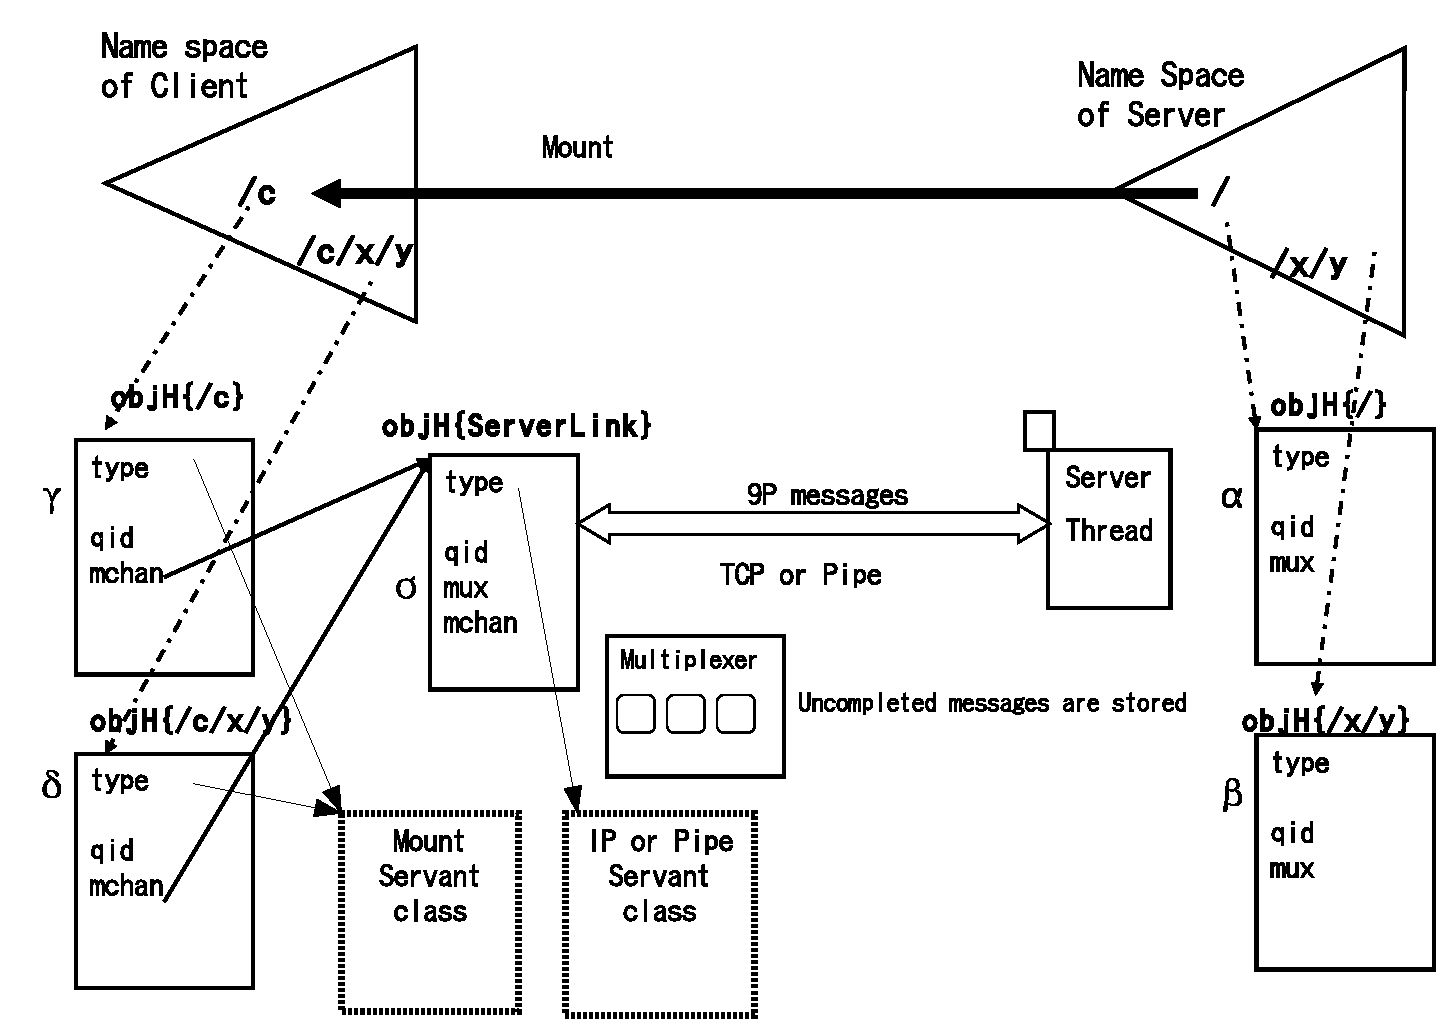
\includegraphics[width=75mm]{../fig/RemoteAccess2.eps}
    \caption{リモートオブジェクトアクセス}
    \label{fig:RemoteAccess}
    \ecaption{Remote object access}
  \end{center}
\end{figure}


%\begin{enumerate}
%\item サーバ登録簿への登録:  
{\bf\flushleft (1) サーバ登録簿への登録: }
  サーバ登録簿にサーバリンクを登録することにより,
  ``{\tt objH\{サーバリンク\}}'' (図の$\sigma$)が割り当てられる.
%
%\item サーバのマウント: 
{\bf\flushleft  (2) サーバのマウント: }
   次の{\tt mount}コマンドによりサーバをマウントする.
   ここに, {\tt /srv/dos}はサーバリンク,
   {\tt /c }はマウントポイント,
   {\tt /dev/sdC0/dos} はサーバ名前空間のマウント開始位置,
   {\tt -ac}は書き込み可能マウントを意味する.

   \verb|mount -ac /srv/dos /c /dev/sdC0/dos|

  LP49coreは,これによりサーバとメッセージのやり取りを行いサーバをマウントする.
  具体的には,
  マウントポイントに``{\tt objH\{/c\}}'' (図の$\gamma$)テーブルを割り付けて,
  サーバ内の``/''オブジェクト(図の$\alpha$)の{\bf Proxyオブジェクト}
  として機能させる,
%
    このテーブルの代表的フィールドの値は次のとおりである: 
    (a) {\tt type}フィールド: マウントサーバント(\verb|#M|).
    (b) {\tt mchan}フィールド: {\tt objH\{サーバリンク\}}.
    (c) {\tt qid}フィールド: サーバ内の開始位置オブジェクトの{\tt qid}.

    こうして,{\tt objH\{/c\}}への操作はマウントサーバントによって
    {\bf 9P メッセージ}に変換され,サーバリンクに送り出される.
   サーバからの返答を受けたらそれをクライアントに返す.
%
%\item サーバ名前空間での操作:  
{\bf\flushleft (3) サーバ名前空間での操作: }
   例えば {\tt /c} にて``{\tt open("x/y", OREAD)}'' を実行したとする.
   LP49coreはサーバとの間で {\tt walk, open}メッセージなどをやり取りして,
   ``{\tt objH\{/c/x/y\}}'' (図の$\delta$)テーブルを割り当てる.
    このテーブルの代表的フィールドの値は次のとおりである:
    (a) {\tt type}フィールド: マウントサーバント(\verb|#M|).
    (b) {\tt mchan}フィールド: {\tt objH\{サーバリンク\}}.
    (c) {\tt qid}フィールド: サーバ内の{\tt /b/c/d}オブジェクト(図の$\beta$)の{\tt qid}.
    つまり,{\tt objH\{/c/x/y\}}はサーバ内の{\tt /x/y}オブジェクト
    の Proxyオブジェクトとなる.
%\end{enumerate}


\subsection{離れた名前空間の可視化}\label{sec:extfs}

リモートノードの任意の部分空間
(そこには複数のサーバントやサーバが接続されていてもよい)
を,自プロセスの名前空間にマウントすることができる.
Plan9 から移植した{\tt extfs}サーバと{\tt import}コマンドが,これを実現する.

{\tt extfs}サーバは,指定された部分名前空間を外部ノードにexportするサーバ,
{\tt import}コマンドはそれを自分の空間にマウントするコマンドである.

例えばリモートホストの {\tt /dev} ディレクトリーをローカルホストにマウントすると,
{\tt /dev} に接続されているリソースにアクセスすることが可能になる.
全てのオブジェクトはファイルインタフェースで操作できるので,
このことはリモートホストのデバイスも操作できることを意味する.

同様にして,{\tt u9fs} というプログラムをUnix上で走らせることにより,
Unixのファイルシステムの部分空間を LP49 上にマウントすることも可能である.
{\tt u9fs}はUnixで9Pプロトコルを理解するプログラムで,
Plan9ユーザグループから移植した.


\subsection{名前空間の機構}

図 \ref{fig:NS-server-servant} に示すように,サーバントやサーバは,
ルートファイルシステム{\bf RootFS}(これもサーバント)を出発点とする名前空間に
接続(マウント)することにより,プロセスに見えるようになる.
Plan9同様に,同一マウントポイントに複数をマウントすることが可能である(unionマウント).
``/dev'' には各種デバイスサーバントが,``/net''にはプロトコルスタックが接続されている.

  Unixではファイルシステムの mount は root 権者のみが行え,
  名前空間は全プロセスで共通である.
  これに対し,Plan9/LP49 の名前空間は,
  各プロセス毎に自前の名前空間({\bf 個別名前空間})を持つことができる.
  名前空間に見えないものはアクセスできないので,緻密なセキュリティー管理を
  実現できる.

\begin{figure}[tb]
  \begin{center}
   %\epsfxsize=340pt
   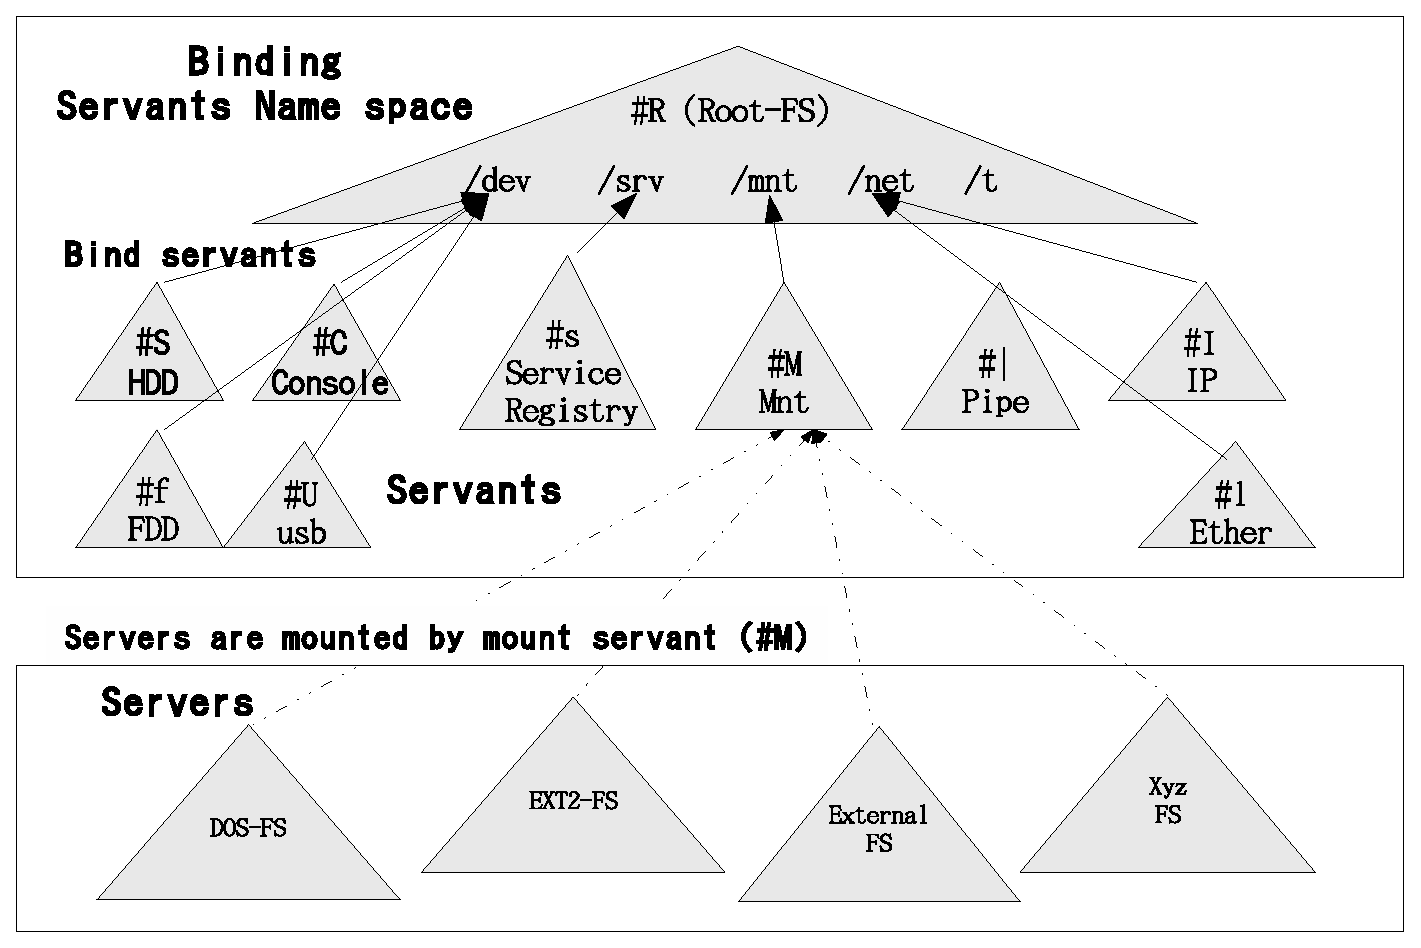
\includegraphics[width=70mm]{../fig/NS-server-servant.eps}
    \caption{サーバ,サーバントと名前空間}
    \label{fig:NS-server-servant}
    \ecaption{Server, servant and Name space}
  \end{center}
\end{figure}


名前空間の構成法を図 \ref{fig:NSmount} に示す.
図中の(a)では,
指定されたマウントポイントにサーバントを結合 (bind) することにより,
サーバントの名前空間がプロセスの名前空間に接続され,
サーバントのサービスを受けられるようになる.

同様に(b)では,サーバーをマウント (mount) することにより,
サーバの名前空間がプロセスの名前空間に接続され,  
サーバのサービスを受けられるようになる.    
サーバは remote procedure call で呼び出されるので,
自ホスト内(b)でもリモートホスト上(c)でも,
同様にアクセスできる.

また,(d)は{\tt extfsサーバ}と{\tt importコマンド}により,
別ノードの``部分''名前空間をマウントしている.

\begin{figure}[tb]
  \begin{center}
   %\epsfxsize=340pt
   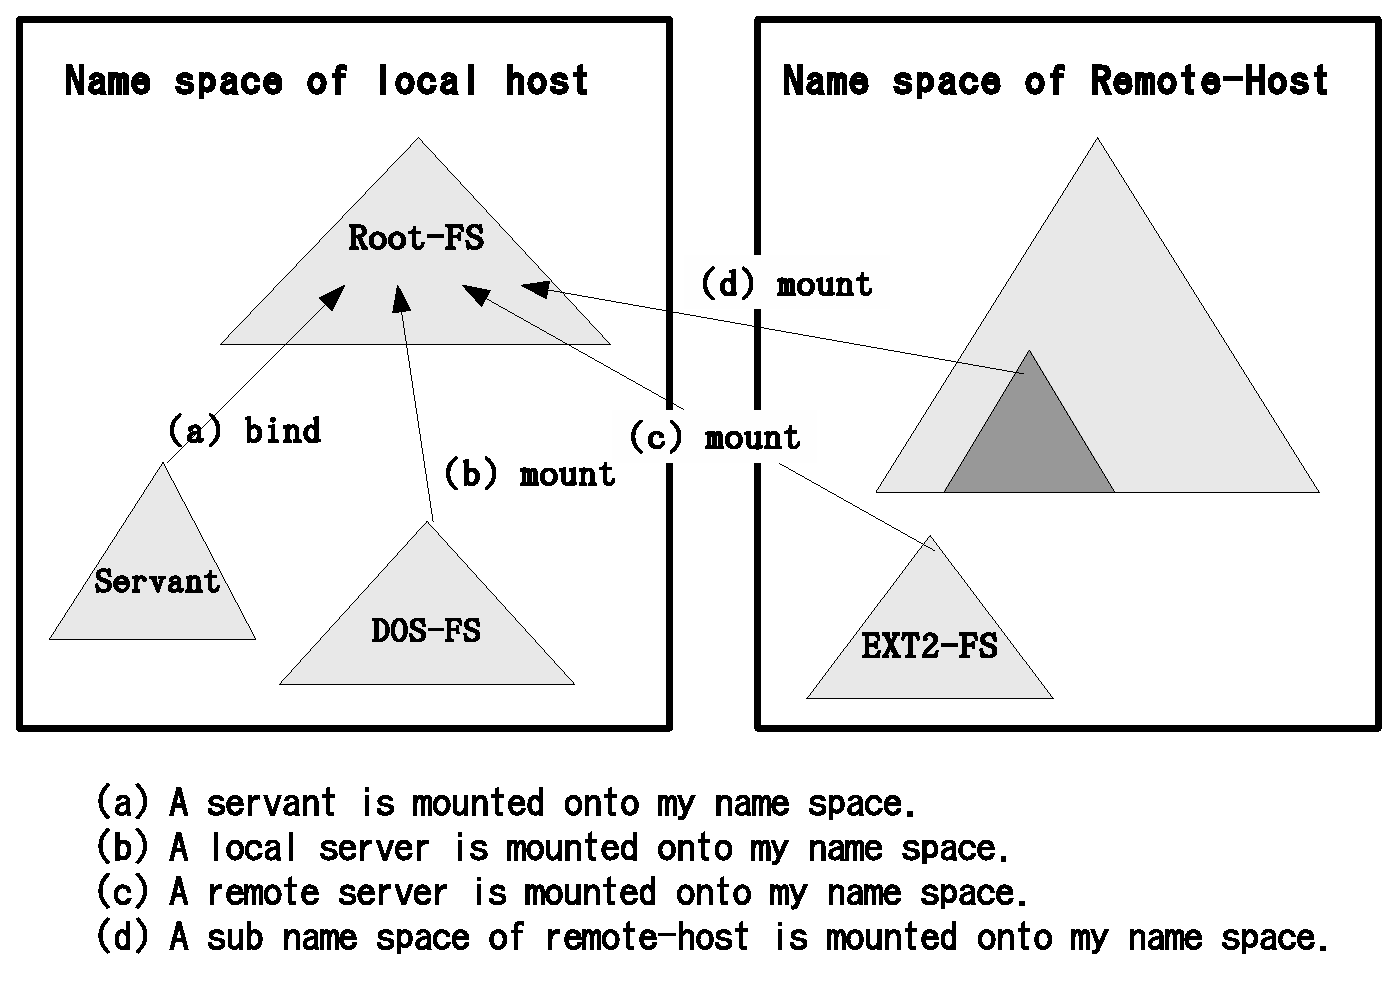
\includegraphics[width=70mm]{../fig/NSmount.eps}
    \caption{名前空間とマウント}
    \label{fig:NSmount}
    \ecaption{Name space and mount}
  \end{center}
\end{figure}


%%%
\subsection{プロトコルスタック}

  Plan9のプロトコルスタックは3回の改良
(Unix system VのStreams型, x-kernel型\cite{xkernel}, 現方式)
 を経ただけに適切にモジュール化されており,
 比較的軽い修正でLP49 に移植することができた.

  インターネットサービスは,
%  図 \ref{fig:NWservants} に示すように
  IPサーバント(``{\tt \#I}'')が提供している.
  IPサーバントの下で
  TCP, UDP, IP など各プロトコル毎にモジュール化されたプログラムが動作しており,
  ユーザには以下のトリー構成をもつファイルシステムとして見える.
  IPサーバントは ``{\tt /net}''に接続され,個々の接続もファイルインタフェースを持つ.
  例えばTCP接続は,{\tt /net/tcp/0, /net/tcp/1 ,,,} として名前空間に見える.

{\footnotesize
\begin{verbatim}

        --+- tcp/ ----+- clone                        
          |           |- stats                
          |           |- 0/ ---+- ctl          
          |           |        |- data     
          |           :        |- local    
          |           :        |           
          |                               
          |- udp/ ---+- clone                        
          |          |- stats                  
          |          |- 0/ ---+- ctl            
          |          |        |-data     
          |          :        |-local    
          |          :        |           
          |                                              
          |-- arp/ ----
\end{verbatim}
}

Etherサーバント(\verb|#l|)は,ether card のサービスインタフェースであり,
該当した ether driver を呼び出している.

\begin{comment}
\begin{figure}[tb]
  \begin{center}
   %\epsfxsize=240pt
   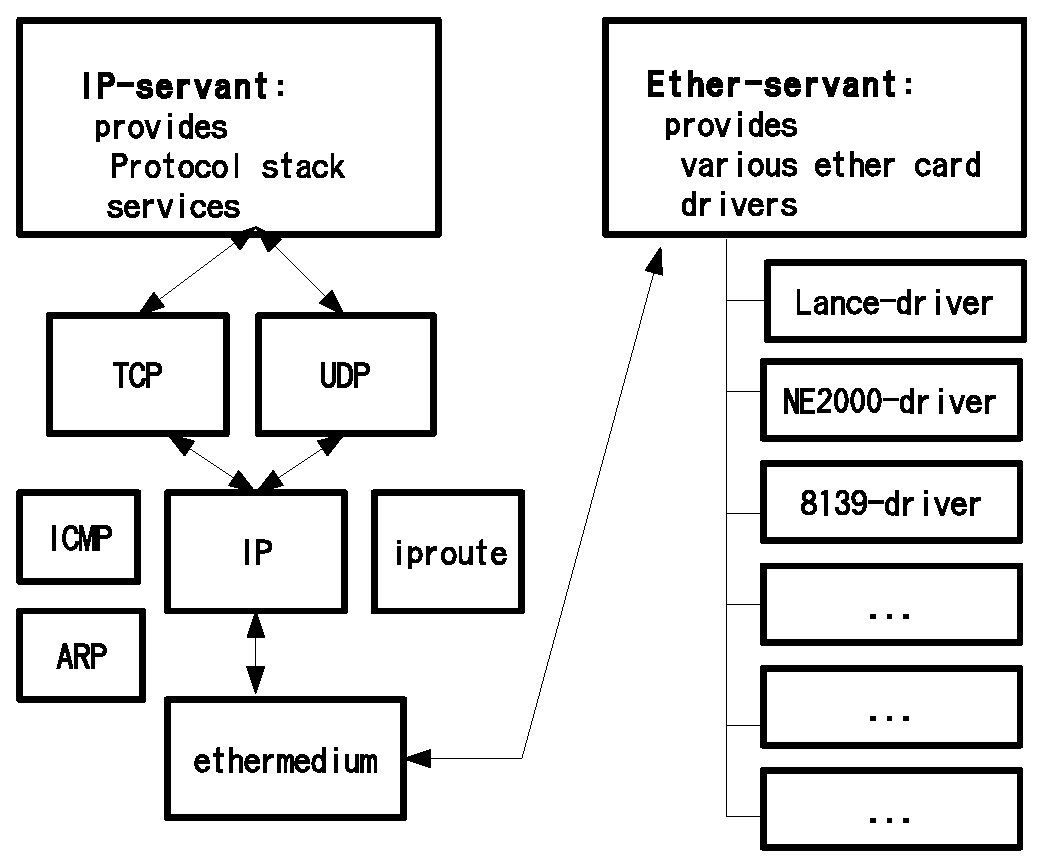
\includegraphics[width=70mm]{../fig/NWservants.eps}
    \caption{IPサーバントとEtherサーバント}
    \label{fig:NWservants}
  \end{center}
\end{figure}
\end{comment}


%}{
\section{本OSキットの開発環境展}

OSの開発および学習には,使い慣れた開発環境が望まれる
(Plan9が普及が遅れている理由には独自の開発環境もある).
またOSの走行テストも,NW機能を含めて実機の前に仮想マシンで行えることが望まれる,

LP49のプログラム開発はLinuxホスト上の GNUツールだけで,
LP49の走行テストはオープンソースエミュレータ Qemu\cite{qemu}で行っている.
%  (図 \ref{fig:SDE}).
Qemu はネットワーク機能も提供しており,
1台のホストマシン上で,
NW接続した複数のLP49を走らせることも,
LP49とLinuxホスト間をNW接続するとも可能である.
1台のホストマシン上で,コンパイルからNWを含む走行試験まで
時間を待たずに行える(単一ソース修正の場合,make してLP49立ち上げまで10
秒程度. 全makeで40秒)ので,大変快適である.

\begin{comment}
\begin{figure}[tb]
  \begin{center}
   %\epsfxsize=400pt
   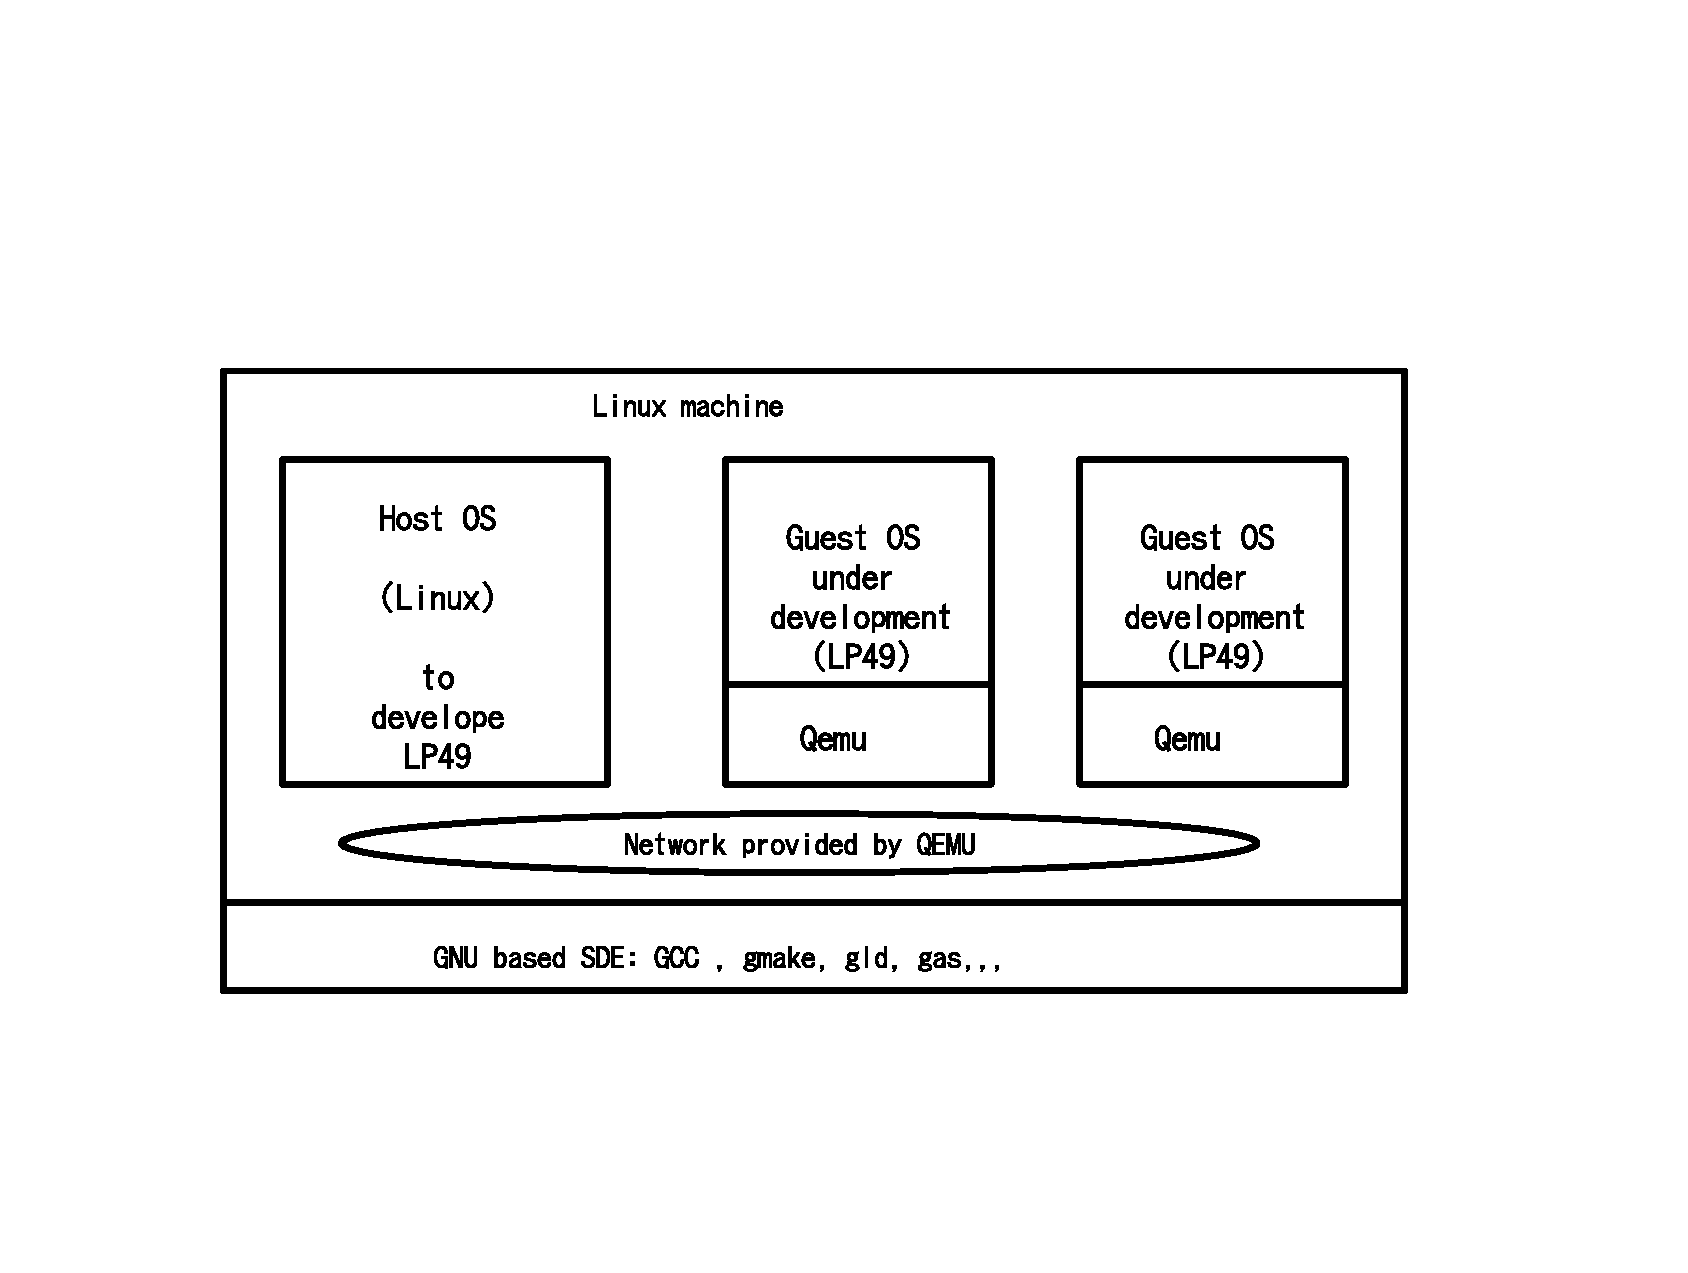
\includegraphics[width=70mm]{../fig/SDE.eps}
    \caption{開発試験環境}
    \label{fig:SDE}
  \end{center}
\end{figure}
\end{comment}

%%%%%%%
\section{関連研究}

% {\bf\flushleft (1) Plan 9}

分散処理機能の観点からは,LP49はPlan9\cite{plan9,plan9HP}の延長にある
開発・学習キットとも云える.
Plan9のソースコードをできる限り活用することとしたが,
実際にはかなりの変更を必要とした(表 \ref{table:LP49-Plan9}).
マイクロカーネル化に伴い,プロセス・スレッド機能とシステムコール機構は
全面的に変更を要した.
プログラム構造的には,マイクロカーネルによる障害保護強化,
サーバントによる部品化強化などを行った.
また,Plan9のサーバとドライバプログラムを少しの修正で移植できた.
9Pプロトコルの採用により,
多くのPlan9サーバを少ない修正でLP49に移植できるという利点もある.
%
Plan9が魅力的な内容にも関わらずハッカーが限られているのは,
%オープンソース化の遅れ(2003年)とともに,
独自のC言語と開発環境が理由と思われる.
特に構造体の無名フィールド (フィールド名を省略でき,
その場合コンパイラがデータタイプから目的フィールドを自動的に探す)
が多用されており,ANSIコンパイラに通らないのみならず,
プログラム解読も難しくしているので,
LP49では人手でプログラム修正
\footnote{GCCへのPlan9-C仕様の追加も考えたが,GCCは改版が頻繁なので断念した.}
を行いGNU環境で開発できるようにした.

\begin{table}[tb]
\caption[Plan9vsLP40]{LP49とPlan9の対比}
\label{table:LP49-Plan9}
\ecaption{LP49 v.s. Plan9}
\begin{center}
{\footnotesize 
\begin{tabular}{l|l|l}
\Hline
 分類  & Plan 9 & LP49 \\
\hline

Micro kernel  &     No        &   Yes   \\
\hline

プロセス  &  コルーチン,     &   L4 Process  \\
スレッド  &  メモリ域共用プロセス &  L4 Thread \\
\hline

システムコール & Trap         &     L4 メッセージ \\
               & プロセスがカーネルモード化   & マルチスレッドサーバ \\
\hline

〃データ入力   & Plan9カーネルが       & L4ページマップ \\
〃データ出力   & APL空間を直接アクセス & L4 ページマップ \\
\hline

ドライバ     & カーネルモード    & ユーザモード  \\
\hline

言語仕様 &  Plan9独自のC言語           &  GCCのC言語  \\
         &  無名フィールド             & \\
         &  typedef, USED(), SET()     &    \\
         &  自動ライブラリリンク       & \\
\hline

コンパイラ &   Plan9独自Cコンパイラ,   &  GCCコンパイラ, \\
 Utility   &   Linker, Assem, mk       &  gld, gas, gmake \\
\hline

Binary    &  a.out形式         &    ELF形式 \\
\Hline

\end{tabular}
}
\end{center}
\end{table}


{\bf L4}\cite{L4,L4HP}は, LP49が採用したマイクロカーネルである.
使い方も容易で,何ら機能追加や修正をすることなく活用できた.

{\bf Minix}\cite{Minix,MinixHP} は学習用マイクロカーネルOSとして,非常に意義が高い.
LinuxはMinixから影響を受けて開発されたが,マイクロカーネルは採用されなかった.
モノリシックOSの方が効率が良いという主張に一理はあるが,
障害に対する頑強性,プログラム保守性はマイクロカーネルが有利である.
Linuxの世界でも最近はユーザレベルファイルサーバが盛んに研究されている.
Minix は分散OS機能は範囲外である.

{\bf SawMil}\cite{SawMill}はIBM で実施されたL4 マイクロカーネルと
マルチサーバからなるOS の研究プロジェクトである.
Linux カーネルをサービス対応にモジュール分けしてマルチサーバ化することを
狙ったが,Linuxカーネルはモジュール分割が困難のため
プロジェクトは中座した.

{\bf $L^4Linux$}\cite{L4Linux}は,L4 マイクロカーネルの上でLinux を動かすOSである.
Linux はモノリシック構成のままであり,L4を使った仮想マシンといえる.

GNU の{\bf Hurd} は,歴史あるマイクロカーネルOS開発である.
マイクロカーネルとしては {\bf Mach}を採用していたが,
効率の観点から最近は L4 マイクロカーネルを採用した{\bf L4-Hurd}\cite{L4Hurd}を検討している.
Unix互換が目標であり,分散OSを目指したものではない.

Microsoft reseach のSIngularity\cite{Singularity}は,安全言語Sing\#の機構で
プロセス保護を行う研究OSである.マルチサーバという点で,同じ方向をめざしている.

%}{

\section{おわりに}

LP49の全ソースコードと資料は,WEBサイト 
http://research.nii.ac.jp/H2O/LP49\cite{LP49HP} にて公開している.
%ソースコードは,更にリファインを進めて簡潔にして行く予定である.

\subsection{今後の展開予定}

{\bf\flushleft (1) 広域サービスバス}

LP49では,OSサービスはサーバもしくはサーバントによって提供される.
LP49coreは,サーバントとサーバのマルチプレクサであり,
APLとサーバやサーバとの間を連携させるメッセンジャーと言える.
% これがシンプル化に役立っている.
ただし,現方式ではシステムコールは全て LP49core を経由して処理されるが,
目的サーバが決まってしまえば
APLとサーバの間で直接メッセージをやり取りさせることもできる.
具体的には,目的サーバの決定に関わるopen(), create(), chdir(),close() を
LP49coreが処理してAPL-サーバ間を安全なチャネルで接続させる.
つまり,OSはサーバを接続するための``広域サービスバス''として
更に簡潔化,融通性強化できる.
これが本研究の最終目的である.

また,9Pプロトコルは同期型メッセージであるが,
広域分散をより効率的に行うために非同期型メッセージもサポートすべく検討中である.
SIP\cite{SIP}プロトコルがVoIPサービスを実現するように,
9Pは分散OSサービスのプロトコルとしての可能性を持っている.
%
{\bf\flushleft (2) 耐障害強化}

プロセスを監視し,障害が見つかればそれを停止して再スタートする仕組みを
組み込む予定である.
また,簡単なPagerの機能追加により,プロセスに保持メモリ域を追加することができる.
保持メモリ域は,プロセス停止後も消去されないメモリセグメントであり,
プロセスが指定した適切なタイミングで無矛盾なデータのスナップショットを書き込んでおく.
プロセスが障害になった場合には,保持メモリ域のデータを使って再開させることにより,
比較的安全なroll backを行える.
%
{\bf\flushleft (3) 最適化}
 
現LP49には,高性能化の仕組みはほとんど組み込んでない.
スレッドの優先度制御,ページキャッシュ,システムコール引数引き継ぎ等の改良で
容易に高性能化を図ることができる.
特にメモリページ割付を担当する Pager の機能拡張を行い,
ページキャッシュ等を実現する予定である.


{\bf\flushleft (4) 認証システム}

分散OSにおいて認証は非常に重要な課題である.
Plan9はKerberos を拡張した精妙な認証方式を実装しているが,
LP49ではIdentity-Based Encryption\cite{IBE}を使用した認証方式の可能性を検討している.


\subsection{OS学習開発キッととして}

{\bf (1) 学習用分散OSとして}

  コメントを含むソース規模は,  
  HVM: 約2K行,LP49core: 約68K行(内19K行がプロトコルスタック),
  ライブラリ: 約19K行,シェル: 約8K行,デバッグシェル: 2K行,
  DosFS: 40K行,Ext2FS: 30K行, extfs: 2K行である.
機能に比べて充分にコンパクトであり,一人で全てをトレースできる.
本キットにより,LP49だけでなく Plan9とL4のプログラム技術も理解できる.


{\bf (2) 分散OS開発キットとして}

コンポーネント化されていること,
大部分の機能追加はサーバ追加で行えること,
サーバはユーザプロセスなので開発が容易なこと,
Plan9のサーバやドライバを容易に移植できることなどの利点がある.

現LP49の測定値は, 実機(Pentium3 1GHz)の場合は以下の通りである.
(a)RAMファイル読み出しは,16B: 21μ sec, 1KB:26μ sec, 4KB:39μ sec, 8KB: 62μ sec.
(b)別マシンのファイル読み出し(\S \ref{sec:extfs}参照)は,
16B:34msec. 1KB: 36msec, 4KB: 54msec, 8KB: 98msec.

QEMU上で走らせた場合(Pentium4 2.8GHz, Fedora8)は以下の通りである.
(a)RAMファイル読み出しは,16B:97μ sec, 1KB:107μ sec, 4KB:157μ sec, 8KB:373μ sec.
(b)別マシンのファイル読み出しは,16B:59ms. 1KB:66msec, 4KB:78msec, 8KB:99msec.

Buffer cacheもpage cacheも未実装なので,
書き込み時間も読み出し時間と殆ど同じである.
まだ充分な最適化は行っていないので性能的には改善の余地があり,
前述のスレッド優先度制御,page cacheなどの導入で性能は向上できる.



% 実機上のLP49のCDファイル(1KB)読み出し時間: 120μ sec.(初回は 110ms). 
% (a)RAMファイル(16B)読み出し時間: 21μ sec.
% (b)RAMファイル(1KB)読み出し時間: 26μ sec.
% (c)RAMファイル(8KB)読み出し時間: 62μ sec.
% (d)別マシンファイル(16B)読み出し時間: 34msec.
% (d)別マシンファイル(1KB)読み出し時間: 36msec.
% (d)別マシンファイル(8KB)読み出し時間: 98msec.
% Qemu上のLP49 -- LP49間のping時間: 4.7ms. 
% Qemu上のLP49 -- Linux/host間のping時間: 0.7ms. 
% Qemu上のLP49 -- LP49間のリモートファイル(1KB)読み出し時間: 40ms. 
% Qemu上のLP49のCDファイル(1KB)読み出し時間: 690μ sec.(初回は 25ms). 
% Qemu上のLP49のRAMファイル(50B)読み出し時間: 180μ sec.
% Qemu上のLP49のRAMファイル(4KB)読み出し時間: 220μ sec.




% \ack
% .....の皆様に,謹んで感謝の意を表する.


%%%
\begin{thebibliography}{10}


\bibitem{plan9}
Rob Pike, et al. : {\em Plan 9 from Bell Labs},Proc. of UKUUG (1991).

\bibitem{plan9HP}
Bell labs.: {\em Plan 9 Web site}, 
http://plan9.bell-labs.com/plan9/

\bibitem{L4}
J. Lidtke: {\em On micro-Kernel Construction}, 
Proc. of IEEE International Workshop on Object-Orientation in Operating Systems (IWOOOS), (1996). 

\bibitem{L4HP}
Karlsruhe univ. : {\em L4 Web site}, 
http://l4ka.org/ 


\bibitem{qemu}
Qemu project : {\em Qemu Web site},\\
http://www.nongnu.org/qemu/ 


\bibitem{Minix}
A. Tannenbaum \& A. Woodhull: {\em Operating systems design and implementation,3/E}, 
Addison-Weisley, (2000).

\bibitem{MinixHP}
www.minix3.org.: {\em Minix  Web site}, 
http://www.minix3.org/

\bibitem{SawMill}
A. Gefflaut, et al.: {\em The SawMill multiserver approach}, 
9th SIGOPS Wuropean Workshop, 2000.

\bibitem{L4Linux}
DROPS OS project : {\em L4Linux Web site}, 
http://os.inf.tu-dresden.de/L4/LinuxOnL4/

\bibitem{L4Hurd}
GNU Hurd project : {\em L4Hurd Web site},\\ 
http://www.gnu.org/software/hurd/history/port\_to\_l4.html


\bibitem{LP49HP}
$H_2O$: {\em LP49  Web site}, 
http://research.nii.ac.jp/H2O/LP49/

\bibitem{xkernel}
N. C. Hutchinson \& L. L. Peterson: 
{\em The x-Kernel: An architecture for implementing network protocols},  
IEEE Transactions on Software Engineering, 17(1), Jan. 1991. 

% \bibitem{Erlang}
% Joe Armstrong: {\em Making reliable distributed systems in the presence of hardware errors}, 
% 博士論文 (Ph.D.) ,スウェーデン王立ストックホルム工科大学, 2003.

\bibitem{Singularity}
G. Hunt. et. al.: {\em An overview of the Singularity Project},
Microsoft research technical report MSR-TR-2005-135, 2005.

\bibitem{SIP}
IETF : {\em RFC 3261: Sessin initial protocol},\\ 
http://tools.ietf.org/html/rfc3261


\bibitem{IBE}
Stanford univ.: {\em Pairing-based cryption library Web site}, 
http://crypto.stanford.edu/pbc/


\end{thebibliography}

%}{

\begin{biography}
\profile*{f}{丸山 勝巳}{昭45東大大学院修士了.同年--平7 電電公社(NTT).
  現在,国立情報学研究所教授.高水準言語,実時間システム,
並行オブジェクト,分散OS等の研究開発に従事.昭57電電公社総裁表彰,
平5情報処理学会論文賞,
平9 電気通信普及財団賞}
\profile*{n}{佐藤 好秀}{%平15東京コンピュータ専門学校卒,
平15年日立製作所入社,平18日立工業専門学院研究科了,
国立情報学研究所にて分散OS研究に従事,現在日立にて金融系SE,}
%

\end{biography}
\end{document}


%%%%%%%%%%
%\ack %% 謝辞

%\bibliographystyle{sieicej}
%\bibliography{myrefs}
%\begin{thebibliography}{99}% 文献数が10未満の時 {9}
%\bibitem{}
%\end{thebibliography}

%\appendix
%\section{}

%\begin{biography}
%\profile{}{}{}
%\profile{会員種別}{名前}{紹介文}% 顔写真あり
%\profile*{会員種別}{名前}{紹介文}% 顔写真なし
%\end{biography}
